\documentclass{DateStructure}

\SubjectName{一元稀疏多项式计算器}
\CollegeName{理学院}
\Major{信息与计算科学}
\GroupNumber{第十六组}

\StudentA{20071226}{童繁}{流程图}
\StudentB{20071227}{王瀚功}{测试}
\StudentC{20071228}{王赛豪}{文案}
\StudentD{20071229}{吴政豪}{调试}
\StudentE{20071230}{武琦}{代码}

\begin{document}
	
\makecover
\newpage

\thispagestyle{empty}
\tableofcontents   

\newpage
\setcounter{page}{1} 
	
\section{需求分析}
\begin{itemize}
\item[(1)]输入并建立多项式;
\item[(2)]输出多项式,输出形式为类数学表达式,序列按指数降序排列;
\item[(3)]多项式A和B相加,建立多项式A+B,输出相加的多项式;
\item[(4)]多项式A和B相减,建立多项式A-B,输出相减的多项式;
\item[(5)]多项式A和B相乘,建立多项式AxB,输出相乘的多项式;	
\item[(6)]计算多项式在$x$处的值;
\item[(7)]求多项式$A$的导函数$A^{'}$;
\item[(8)]设计一个菜单,具有上述操作要求的基本功能。
\end{itemize}

\section{概要设计}
要设计一个一元稀疏多项式简单计算器,可以用两个带表头节点的单链表A、B分别存储两个多项式,进行初步整理——排序和同指数项相加。下列是具体运算算法:\par
1.做加法时,将A链和B链的所有结点都添加到新链C中;\par
2.做减法时,将B链的所有结点的系数变为相反数后与A链进行加法运算,再将B链变回原链表以便重复使用;\par
3.做乘法时,遍历A链的所有结点,遍历B链的所有结点,也就是双重循环,将A*B的所有结点添加到新链C中;\par
4.求导时,将求导后的所有结点添加到新链C中。\par
进行以上运算时,首先建立一个新的链表C,实行相应的算法,在运算结束后输出的新链表C即为最终结果。而将x代入多项式求值时,只需将x代入每项求值,再求和后输出最终结果。\par
\begin{figure}[H]
\centering
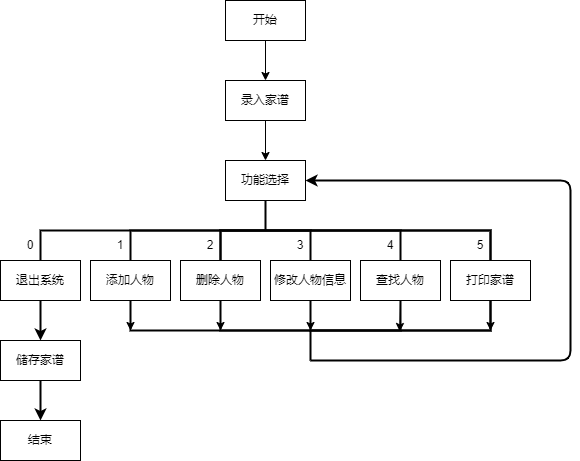
\includegraphics[width=500pt]{main.png}
\caption{主函数流程图}
\end{figure}

\section{详细设计}
要解决上述问题,我们设计了9个函数,流程图和函数代码如下:\par		
\subsection{创建链表}
\begin{figure}[H]
\centering
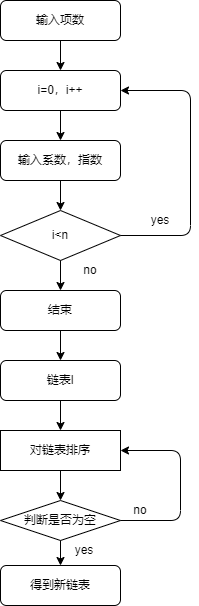
\includegraphics[width=150pt]{创建链表.png}
\caption{链表创建流程图}
\end{figure}
\subsubsection{输入多项式}
\begin{lstlisting}[language=c,caption={input}]
list input() //函数:输入多项式
{
	list a,b,l;
	l=(list)malloc(sizeof(node));
	l->next=NULL;
	b=l;
	int n,i;
	printf("请输入项数:");
	scanf("%d",&n);//输入项数
	printf("请输入系数 指数:\n");
	for(i=0;i<n;i++)
	{
		a=(list)malloc(sizeof(node));
		printf("第%d项:",i+1);
		scanf("%lf %d",&(a->coe),&(a->exp));//输入系数和指数
		a->next=NULL;
		b->next=a;
		b=a;
	}
	return l;
}
\end{lstlisting}
\subsubsection{多项式整理}
\begin{lstlisting}[language=c,caption={sort}]
void sort(list l)//多项式整理
{
	list i,j;
	double tcoe;
	int texp;
	for(i=l->next;i!=NULL;i=i->next)
	{
		for(j=i->next;j!=NULL;j=j->next)
		{
			if(j->exp>i->exp)
			{
				tcoe=j->coe;
				j->coe=i->coe;
				i->coe=tcoe;
				texp=j->exp;
				j->exp=i->exp;
				i->exp=texp;
			}
			else if(j->exp==i->exp)
			{
				tcoe=j->coe+i->coe;
				i->coe=tcoe;
				j->coe=0;
				i->exp=j->exp;
				j->exp=0;
			}
		}
	}
}		
\end{lstlisting}
\subsection{输出多项式}
\begin{figure}[H]
\centering
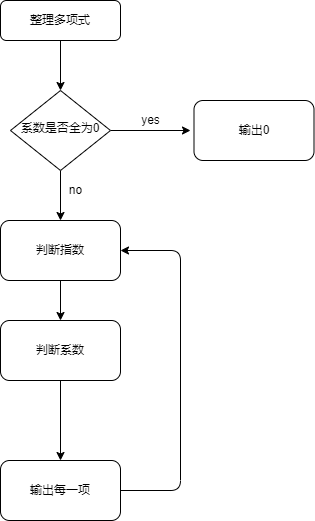
\includegraphics[width=150pt]{输出多项式.png}
\caption{多项式输出流程图}
\end{figure}
\begin{lstlisting}[language=c,caption={output}]
void output(list l)//函数:输出多项式
{
	sort(l);
	list a,b;
	int i=0,j=0,k=0;
	a=l->next;
	b=l->next;
	while(b)
	{
		j++;
		if(b->coe==0.0)
			k++;
		b=b->next;
	}
	if(j==k)
		printf("0");
	else
	{
		while(a)
		{
			if(a->exp!=0)
			{
				if(a->coe<0)
				{
					printf("-");
					if(a->exp==1)
					{
						if(a->coe==-1)
							printf("x");
						else
							printf("%.*lfx",m,-a->coe);
					}
					else
					{
						if(a->coe==-1)
							printf("x^%d",a->exp);
						else
							printf("%.*lfx^%d",m,-a->coe,a->exp);
					}
				}
				else if(a->coe>0)
				{
					if(i!=0)
						printf("+");
					if(a->exp==1)
					{
						if(a->coe==1)
							printf("x");
						else
							printf("%.*lfx",m,a->coe);
					}
					else if(a->exp!=1)
					{
						if(a->coe==1)
							printf("x^%d",a->exp);
						else
							printf("%.*lfx^%d",m,a->coe,a->exp);
					}
				}
			}
			else
			{
				if(a->coe<0)
					printf("%.*lf",m,a->coe);
				else if(a->coe>0)
				{
					if(i==0)
						printf("%.*lf",m,a->coe);
					else
						printf("+%.*lf",m,a->coe);
				}
			}
			a=a->next;
			i++;
		}
	}
	printf("\n");
}
\end{lstlisting}
\subsection{加法}
\begin{figure}[H]
\centering
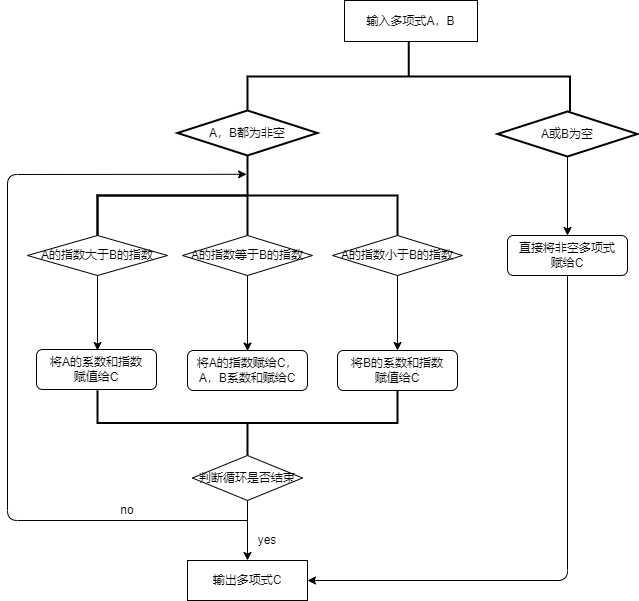
\includegraphics[width=300pt]{加法.png}
\caption{加法流程图}
\end{figure}
\begin{lstlisting}[language=C,caption={plus}]
void plus(list a,list b)//函数:多项式相加
{
	list la,lb,lc,ld,c,d;
	c=(list)malloc(sizeof(node));
	c->next=NULL;
	d=c;
	la=a->next;
	lb=b->next;
	while(la!=NULL&&lb!=NULL)
	{
		lc=(list)malloc(sizeof(node));
		lc->next=NULL;	
		if(la->exp>lb->exp)
		{
			lc->exp=la->exp;
			lc->coe=la->coe;
			d->next=lc;
			d=lc;
			la=la->next;
		}
		else if(la->exp==lb->exp)
		{
			double sum=la->coe+lb->coe;
			if(sum!=0.0)
			{
				lc->exp=la->exp;
				lc->coe=sum;
				d->next=lc;
				d=lc;
			}
			la=la->next;
			lb=lb->next;
		}
		else
		{
			lc->exp=lb->exp;
			lc->coe=lb->coe;
			d->next=lc;
			d=lc;	
			lb=lb->next;			
		}			
	}
	while(la)
	{
		lc=(list)malloc(sizeof(node));
		lc->next=NULL;	
		lc->exp=la->exp;
		lc->coe=la->coe;			
		la=la->next;
		d->next=lc;
		d=lc;
	}
	while(lb)
	{
		lc=(list)malloc(sizeof(node));
		lc->next=NULL;	
		lc->exp=lb->exp;
		lc->coe=lb->coe;
		lb=lb->next;
		d->next=lc;
		d=lc;	
	}
	output(c);
}		
\end{lstlisting}
\subsection{减法}
\begin{figure}[H]
\centering
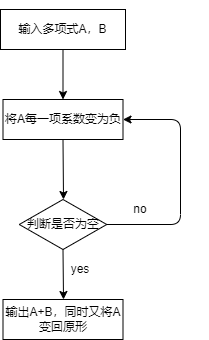
\includegraphics[width=150pt]{减法.png}
\caption{减法流程图}
\end{figure}
\subsubsection{多项式系数变负}
\begin{lstlisting}[language=C,caption={oppo}]
void oppo(list *l)//函数:多项式系数变负
{
	list a=(*l)->next;
	while(a)
	{
		a->coe=-a->coe;
		a=a->next;
	}
}
\end{lstlisting}
\subsubsection{减法}
\begin{lstlisting}[language=C,caption={minus}]
void minus(list a,list b)//函数:多项式相减
{
	oppo(&b);
	plus(a,b);
	oppo(&b);
}
\end{lstlisting}
\subsection{乘法}
\begin{figure}[H]
\centering
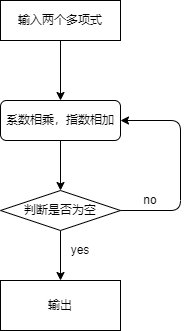
\includegraphics[width=150pt]{乘法.png}
\caption{乘法流程图}
\end{figure}
\begin{lstlisting}[language=C,caption={multi}]
void multi(list a,list b)//函数:多项式乘法
{
	list la,lb,lc,c,ld;
	la=a->next;
	lb=b->next;
	c=(list)malloc(sizeof(node));
	lc=c;
	lc->next=NULL;
	while(la)
	{
		lb=b->next;
		while(lb)
		{
			ld=(list)malloc(sizeof(node));
			ld->next=NULL;
			ld->coe=la->coe*lb->coe;
			ld->exp=la->exp+lb->exp;
			lc->next=ld;
			lc=ld;
			lb=lb->next;
		}
		la=la->next;
	}
	output(c);
}
\end{lstlisting}
\subsection{赋值运算}
\begin{figure}[H]
\centering
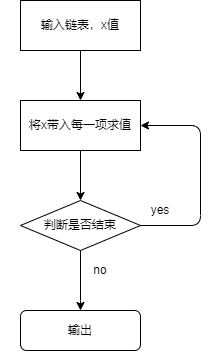
\includegraphics[width=150pt]{求在x处的值.png}
\caption{赋值运算流程图}
\end{figure}
\begin{lstlisting}[language=C,caption={fx}]
void fx(list a,double x)//函数:多项式在x处的值
{
	list la;
	la=a->next;
	double value=0;
	while(la)
	{
		value+=(la->coe)*pow(x,la->exp);
		la=la->next;
	}
	printf("在%.*lf处的值为:%.*lf\n",m,x,m,value);
}
\end{lstlisting}	
\subsection{求一阶导}
\begin{figure}[H]
\centering
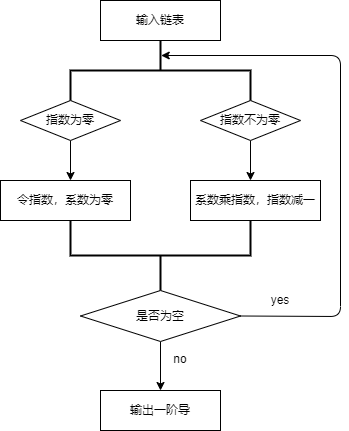
\includegraphics[width=200pt]{求一阶导.png}
\caption{求导流程图}
\end{figure}
\begin{lstlisting}[language=C,caption={diff}]
void diff(list a)//函数:求一阶导
{
	list la,b,lb,lc;
	la=a->next;
	b=(list)malloc(sizeof(node));
	lb=b;
	lb->next=NULL;
	while(la)
	{
		lc=(list)malloc(sizeof(node));
		if(la->exp==0)
		{	
			lc->coe=0.0;
			lc->exp=0;
		}
		else
		{
			lc->coe=la->coe*la->exp;
			lc->exp=la->exp-1;
		}
		lc->next=NULL;
		lb->next=lc;
		lb=lc;
		la=la->next;
	}
	printf("的一阶导为:");
	output(b);
}
\end{lstlisting}		

\section{测试案例}
例1:$(2x+5x^{8}-3.1x^{11})+(7-5x^{8}+11x^{9})=-3.1x^{11}+11x^{9}+2x+7$\par
\begin{figure}[H]
\centering
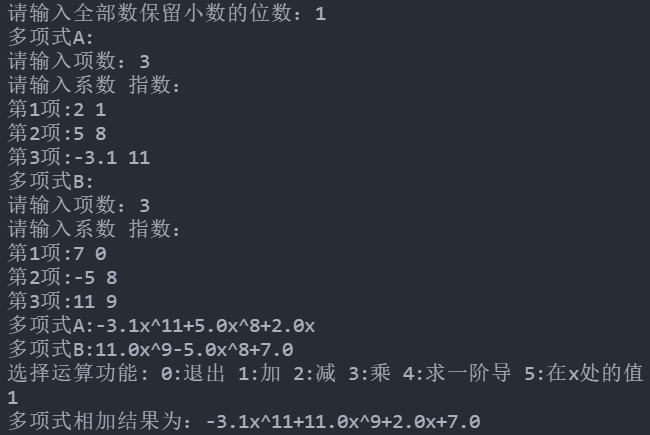
\includegraphics[width=400pt]{测试1.png}
\caption{测试1}
\end{figure}	
例2:$(6x^{-3}-x+4.4x^{2}-1.2x^{9})-(-6x^{-3}+5.4x^{2}-x^{2}+7.8x^{15})=-7.8x^{15}-1.2x^{9}-x+12x^{-3}$\par
\begin{figure}[H]
\centering
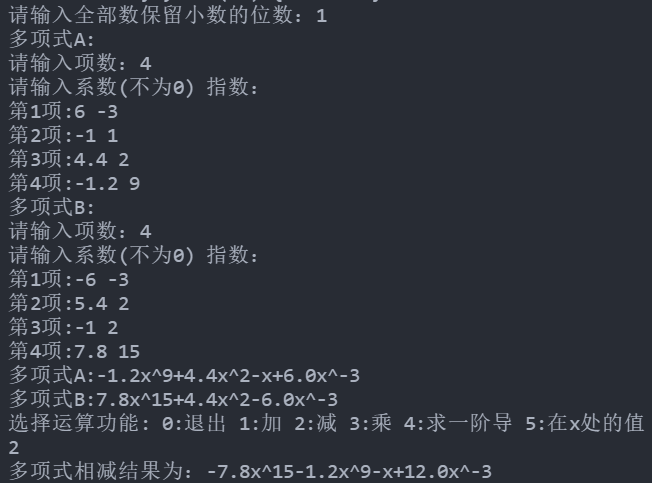
\includegraphics[width=400pt]{测试2.png}
\caption{测试2}
\end{figure}
例3:$(1+x+x^{2}+x^{3}+x^{4}+x^{5})+(-x^{3}-x^{4})=x^{5}+x^{2}+x+1$\par
\begin{figure}[H]
\centering
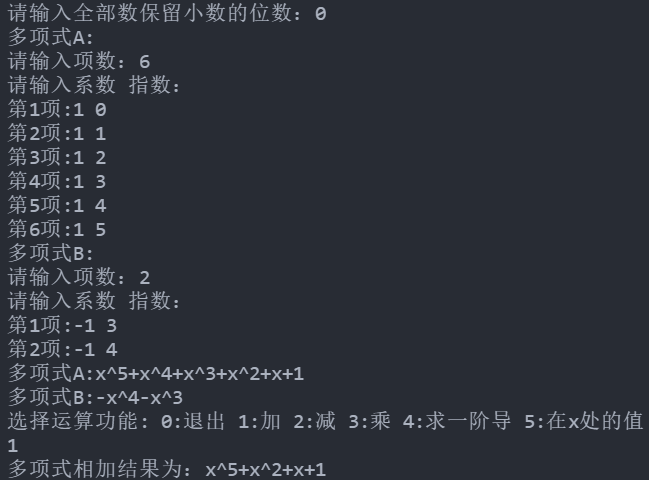
\includegraphics[width=400pt]{测试3.png}
\caption{测试3}
\end{figure}
例4:$(x+x^{3})+(-x-x^{3})=0$\par
\begin{figure}[H]
\centering
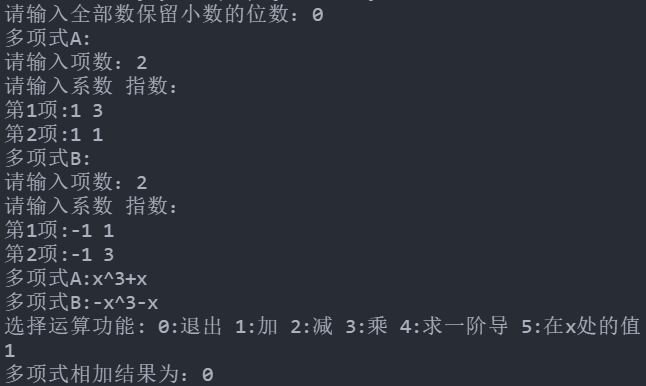
\includegraphics[width=400pt]{测试4.png}
\caption{测试4}
\end{figure}
例5:$(x+x^{100})+(x^{100}+x^{200})=x^{200}+2x^{100}+x$\par
\begin{figure}[H]
\centering
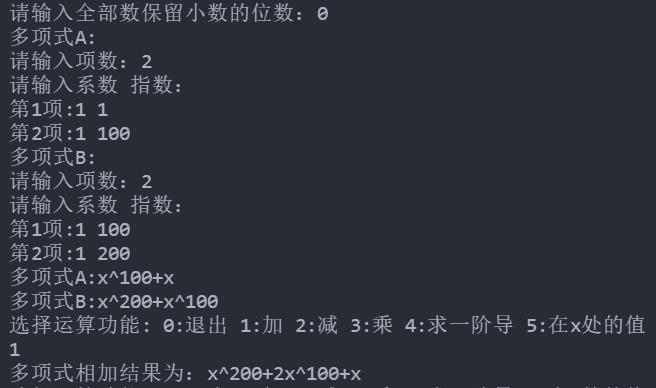
\includegraphics[width=400pt]{测试5.png}
\caption{测试5}
\end{figure}
例6:$(x+x^{2}+x^{3})+0=x^{3}+x^{2}+x$\par
\begin{figure}[H]
\centering
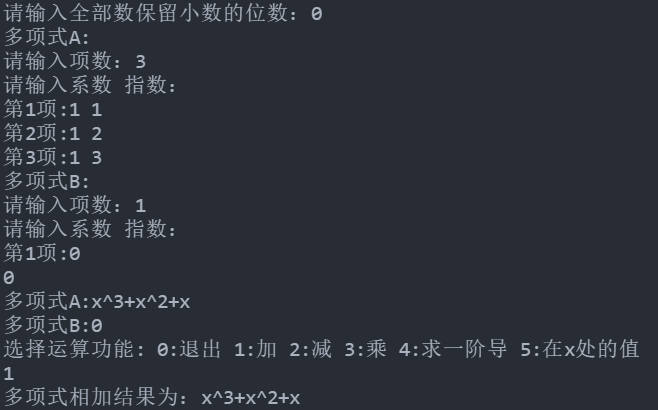
\includegraphics[width=400pt]{测试6.png}
\caption{测试6}
\end{figure}
\section{功能测试}
例一:$A:3x^{4}+0.002x^{3}-2x^{2}+13x+1\quad B:5x^{6}+2x^{3}-0.3x^{2}-12$\par
\begin{figure}[H]
\centering
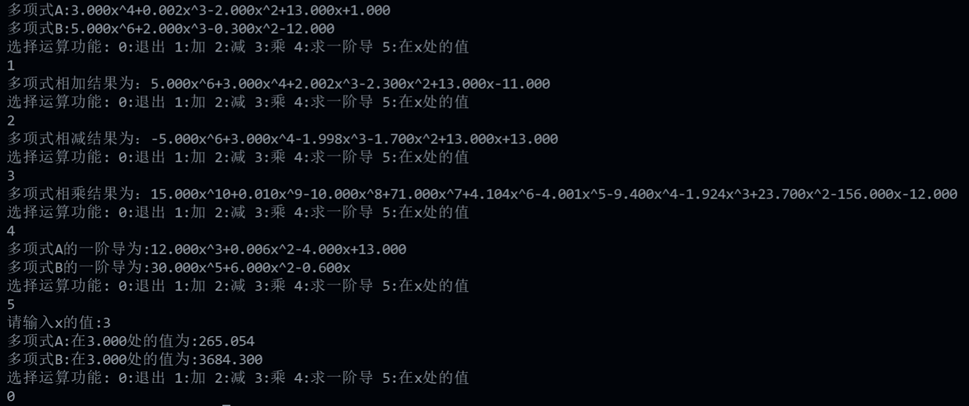
\includegraphics[width=400pt]{功能测试1.png}
\caption{功能测试1}
\end{figure}
例二:$A:2x^{3}+x^{2}+x-1\quad B:-2x^{4}+x^{3}+2x$\par
\begin{figure}[H]
\centering
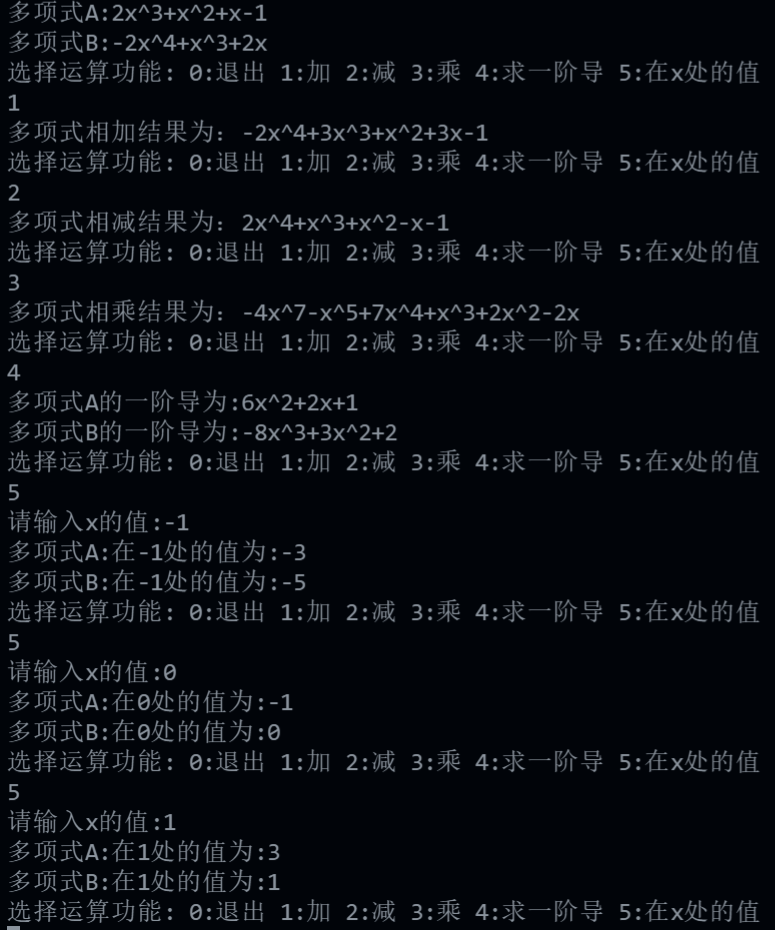
\includegraphics[width=400pt]{功能测试2.png}
\caption{功能测试2}
\end{figure}
例三:$A:0.3x^{2}-0.04x+0.005\quad B:-0.3x^{2}+0.04x+0.005$\par
\begin{figure}[H]
\centering
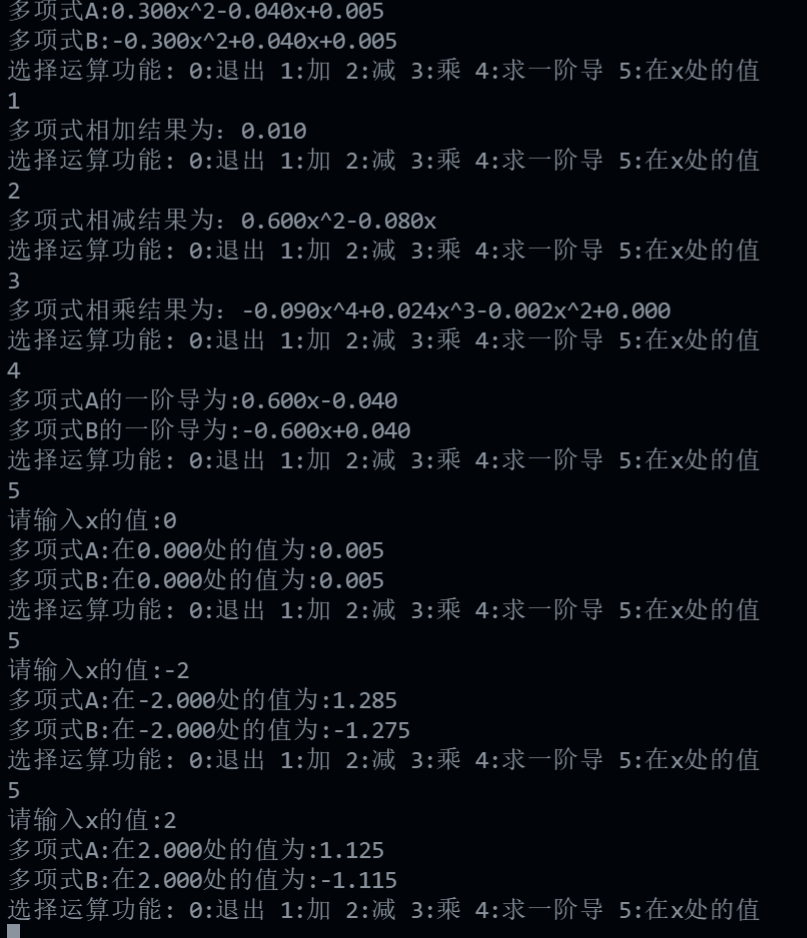
\includegraphics[width=400pt]{功能测试3.png}
\caption{功能测试3}
\end{figure}

\newpage 
\section{附录}
\lstinputlisting[language=C]{main.c}
\end{document}
